
\chapter{Jak predikovat přítomnost: mobilita, internetové vyhledávání etc.}
\label{Predikce_pritomnosti}

\textit{Autor První, Autor Druhý, Autor Další}
\vspace{15mm}

   Při psaní článku používáme strukturu výzkumného článku IMRAD \cite{tulinska}. V~úvodu článku by měl být uveden současný stavv poznání \cite{colu92} a skutečnosti, které jsou základem pro další text \cite{phil99} s~přihlédnutím ke srozumitenosti celého textu pro čtenáře mimo obor.


\section*{Úvod} 

Úvod skutečně uvádí čtenáře do problematiky vaší práce. To znamená, že je potřeba vysvětlit motivaci pro zkoumání tématu a jeho přínos a uvést otázku či otázky, které jste si kladli.  

Součástí úvodu (nebo za ním) je uvedení kontextu. To znamená najít relevantní autory a studie, které se dané oblasti věnují, a popsat, jak k~ní přistupují a s~jakými výsledky.  

Je zde také potřeba vysvětlit, jak chápete danou oblast. To se někdy dělá s~využitím slovníkových definic, což ale nemusí být nutně nejlepší strategie – definice zastupují jakousi převládající představu o~dané věci. Můžete jít i jinou cestou, totiž popisováním pomocí vybraných autorů a jejich myšlenek, ze kterých vyplývá také vaše uchopení a vidění věci. 

    Jaké je téma, cíl, řešený problém práce? Proč má smysl se jím zabývat? 
    Jaký je současný stav poznání? Kdo o~něm píše a co? 
    Jakou výzkumnou otázku jste si kladli? 

\section*{Metody} 

V~metodách je potřeba čtenáři srozumitelně sdělit, jakým způsobem jste došli k~výsledkům. Postup byste měli popsat co nejlépe. Ukazuje to totiž na objektivitu a z~toho pramenící důvěryhodnost vámi předkládaných informací. V~podstatě stačí odpovědět na těchto šest otázek: 

    Jak jste na ni odpovídali? Pomocí kvalitativních nebo kvantitativních metod? 
    Jaké nástroje vám k~tomu pomohly? Rozhovor či dotazník?
    Jak jste data sbírali? Jak jste vybrali lidi, kterých jste se ptali? 
    Jaký byl vzorek? Koho přesně jste se ptali a proč zrovna jich, v~jakém počtu? 
    Jak jste data zpracovali? Tedy co jste s~rozhovory či dotazníkem udělali? 
    Jak jste se postarali o~etiku výzkumu? Například o~to, aby byl dotazník anonymní? 

\section*{Výsledky} 

Ve výsledcích sepíšete, co jste se danou metodou dověděli. To znamená, kolik procent studentů odpovědělo v~dotazníku na danou otázku nebo co lidé řekli, když jste se jich na tuto otázku ptali. Pozor – nevejde se tady zřejmě vše, co jste zjistili. Ze svých dat vybíráte ta, která nejvíce odpovídají vašemu cíli a zodpovězení vaší otázky. 

    Jaká data jste získali? Jaké odpovědi? 
    Jak souvisí se zodpovězením vaší otázky? 

\section*{Analýza a diskuse} 

Analýza a diskuse se zabývá výsledky. U~kvalitativního výzkumu mohou být tyto části spojené. Znamená to, že se nyní podíváte na to, co jste zjistili a zkoušíte vyvodit, co to znamená, s~čím to souvisí, na co to ukazuje. Hrajete si s~myšlenkami a odkazujete na zdroje, které jste na četli. Souvisí to s~nimi? Souhlasí? Odporuje?  
Závěr 

V~závěru je za potřebí pomoci čtenáři uzavřít myšlenky, kterými jste ho provázeli. Co tedy vyplynulo? Co jsou tři nejpodstatnější věci? Závěr by měl kamarádit s~úvodem – pokud by někdo přečetl jen tyto dvě části, stejně by měl pochopit to hlavní, o~čem text je. 

\section*{Příloha}
Nepředpokládá se, že by součástí textu pro monografii byly nějaké přílohy, zde jsou uvedeny pouze jako příklady, sazby základních prvků, kterých je při psaní textu třeba. Následují příklady použití prostředí pro vkládání obrázků, tabulek a matematických vzorců.

\subsection*{Vkládání obrázků}

Na obrázku \ref{fig:140-krivky_pokriv} jsou k~vidění dvě osy nebarevné a čtyři křivky barevné.

\begin{figure}[ht]
    \centering
    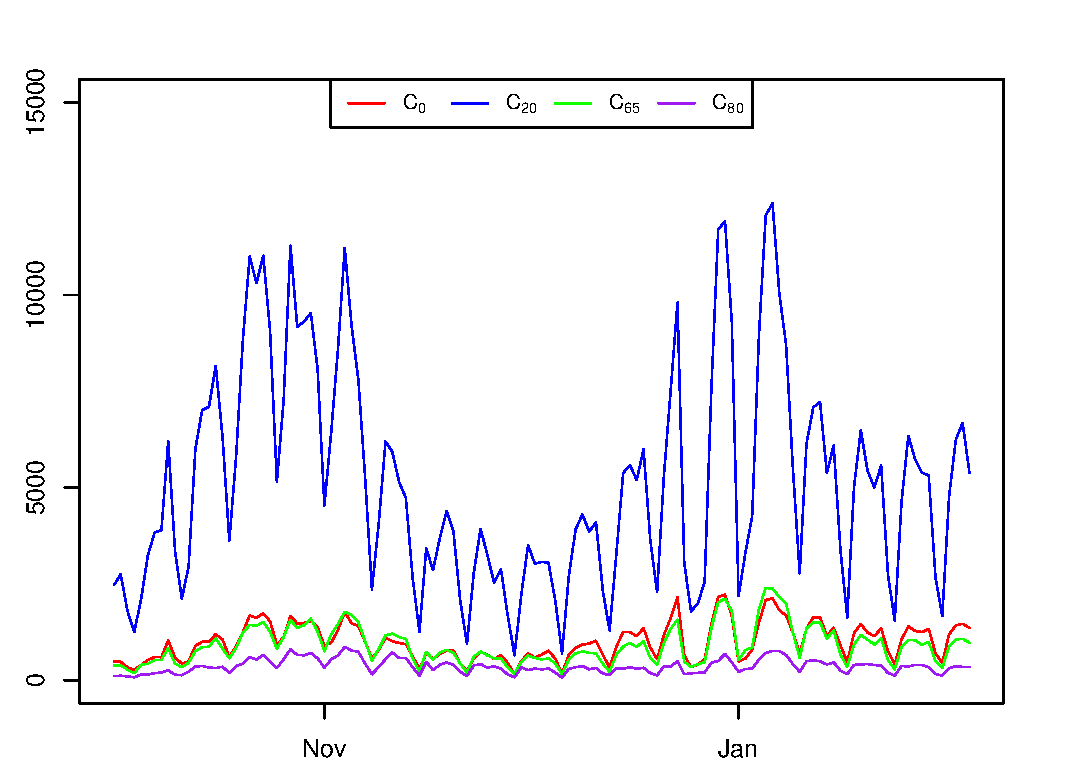
\includegraphics[width=200pt]{./pic/140-C0-80.eps}
    \caption{Křivky pokřivené}
    \label{fig:140-krivky_pokriv}
\end{figure}


\subsection*{Vkládání tabulky}

V~nálsedujícím testu bude vložena tabulka \ref{tab:140-test}, tabulka jest definována prostředím tabular. Na adrese \url{https://www.overleaf.com/learn/latex/Tables} je dostupný návod jak s~tabukami pracovat. Celé prostředí tabular je obaleno blokem table, který umožňuje definovat polohu tabulky na stránce a vložit k~tabulce popisek a značku label pro referenci v~textu.


\begin{table}[h]
    \centering
    \caption{Kódy jednotlivých států použité v~číselníku}
\begin{tabular}{ p{3cm} p{2cm} p{2cm} p{2cm}  }
 \hline
 \multicolumn{4}{ c }{Country List} \\
 \hline
 Country Name     or Area Name& ISO ALPHA 2 Code &ISO ALPHA 3 Code&ISO numeric Code\\
 \hline
 Afghanistan   & AF    &AFG&   004\\
 Aland Islands&   AX  & ALA   &248\\
 Albania &AL & ALB&  008\\
 \hline
\end{tabular}
    
    \label{tab:140-test}
\end{table}

\subsection*{O dalších prvcích textu}

Odstavce se oddělují prázdným řádkem. Vzhledem k~tomu, že text bude převáděn do výsledné grafické podoby, snažte se vyhnout zbytečnému používání \emph{zvýrazněním} a jiným \textbf{grafickým úpravám} textu. Čím více se článek bude blížit čistému textu, tím lépe z~hlediska dalšího zpracování příspěvku před finální sazbou. Grafické uspořádání textu po kompilaci je pouze náhledem, nikoli výslednou grafickou podobou.

V~textu je možné - je-li to nutné - používat i matematické vzorce \ref{140-kombin_c}, pro které slouží prostředí equation.

\begin{equation}
    \label{140-kombin_c}
    \binom{n}{k} = \frac{n!}{k!(n-k)!}
\end{equation}

Pokud uznáte za vhodné použít poznámku pod čarou\footnote{Autorova slabost pro používání poznámek pod čarou je způsobena především těkavostí a snahou sdělit alespoň významnější širší souvislosti.}, můžete tak učinit.

Pro zápis do záznamů použivejte syntaxi uvedenou na stránkách: \url{http://bib-it.sourceforge.net/help/fieldsAndEntryTypes.php}